%\newpage
%\section{Resultados}
%
%\subsection{Modulação M-ASK}
%Foi colocado as ponteiras nos lugares demarcados segundo a figura \ref{fig:ASK} e obteve-se a seguinte sequência de gráficos nos pontos onde se tinha osciloscópios:
%
%\begin{figure}[H]
%    \centering
%    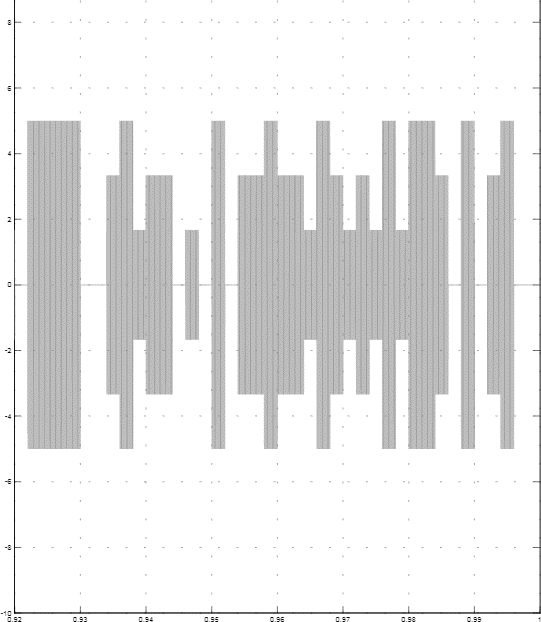
\includegraphics[scale=0.4]{rask1}
%    \caption{ASK.}
%    \label{fig:rask1}
%\end{figure}
%
%\begin{figure}[H]
%    \centering
%    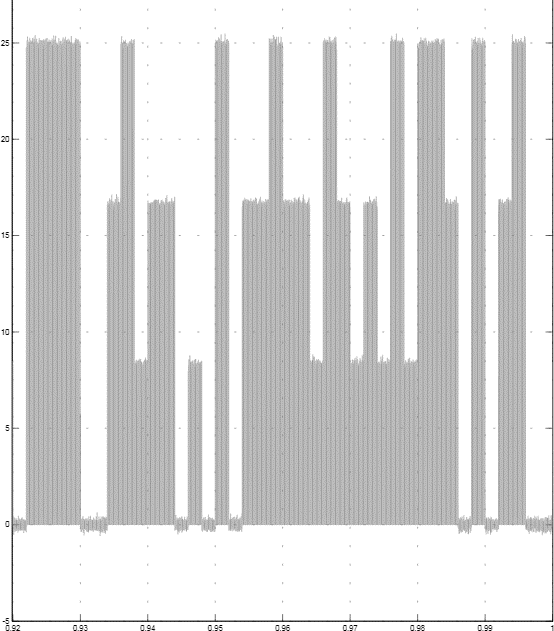
\includegraphics[scale=0.4]{rask2}
%    \caption{ASK1.}
%    \label{fig:rask2}
%\end{figure}
%
%\begin{figure}[H]
%    \centering
%    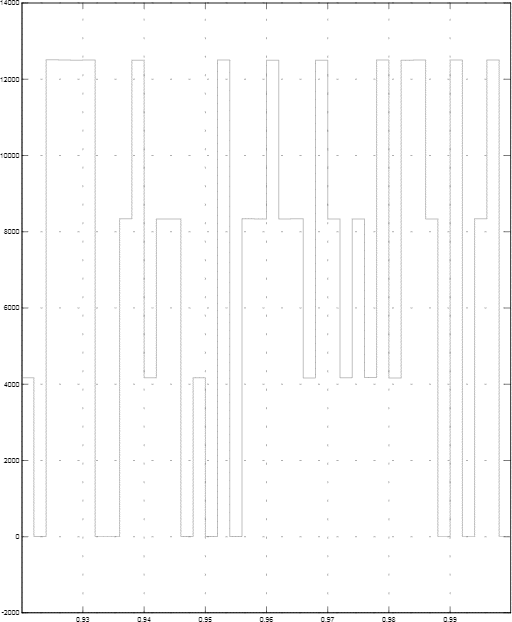
\includegraphics[scale=0.4]{rask3}
%    \caption{ASK2.}
%    \label{fig:rask3}
%\end{figure}
%
%\begin{figure}[H]
%    \centering
%    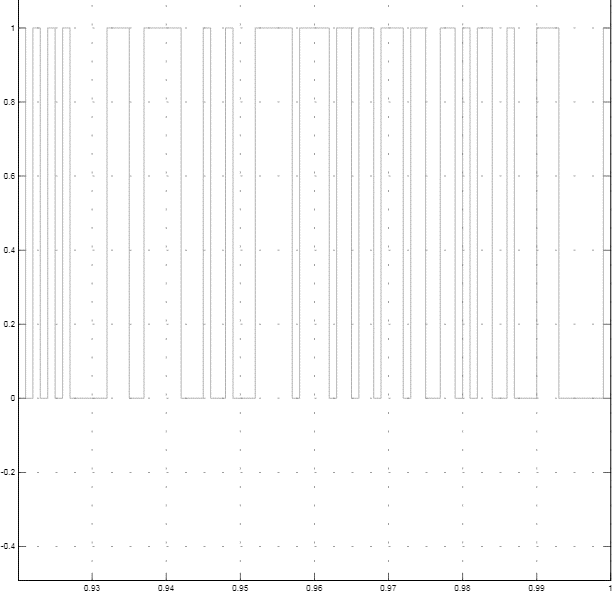
\includegraphics[scale=0.4]{rask4}
%    \caption{ASK3.}
%    \label{fig:rask4}
%\end{figure}
%
%\begin{figure}[H]
%    \centering
%    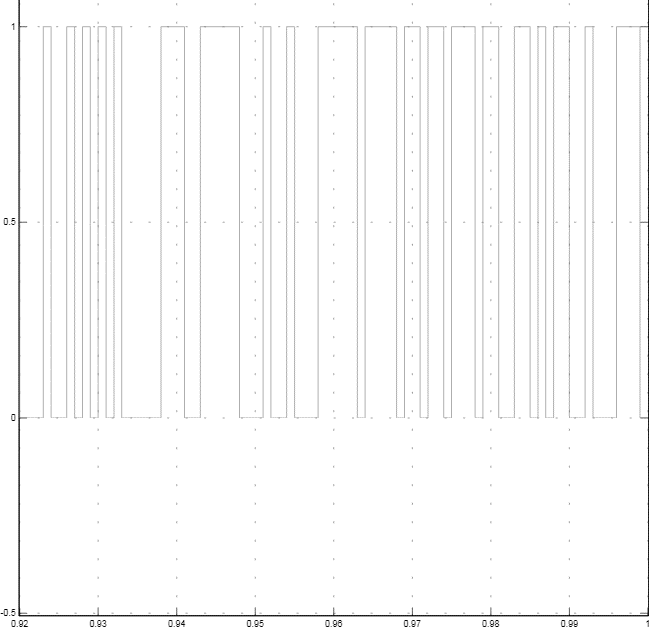
\includegraphics[scale=0.4]{rask5}
%    \caption{ASK4.}
%    \label{fig:rask5}
%\end{figure}
%
%Para ser verificado o atraso no sinal recebido em relação ao transmitido, verificou-se pela figura \ref{fig:rask6}, que temos um atraso de 6 bits da entrada em relação a saída:
%\begin{figure}[H]
%    \centering
%    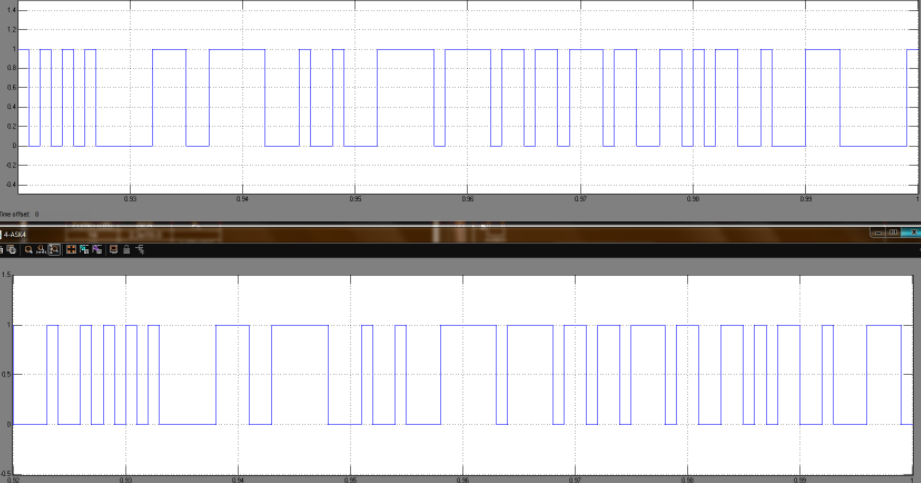
\includegraphics[scale=0.3]{rask6}
%    \caption{Atraso.}
%    \label{fig:rask6}
%\end{figure}
%
%
%Obteve-se então o seguinte gráfico relacionando os resultados práticos (BER) e os teóricos (PB), de acordo com a tabela acima apresentada:
%
%\begin{figure}[H]
%    \centering
%    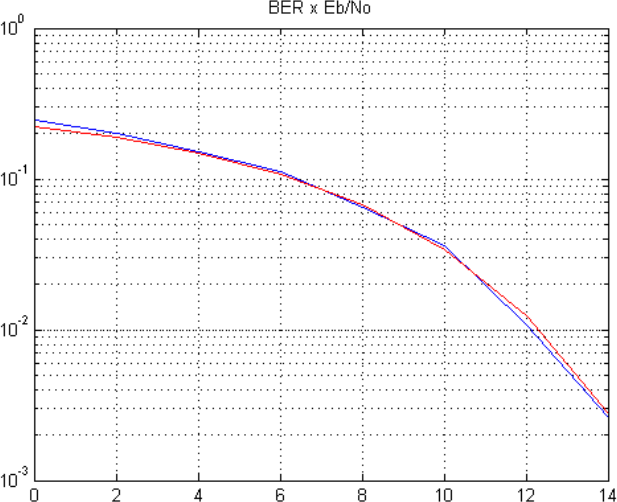
\includegraphics[scale=0.3]{rask7}
%    \caption{Relação BERxNo e Pb.}
%    \label{fig:rask7}
%\end{figure}
%
%Também encontrou-se a relação ASK com ASK4 e ASK2 com ASK1, sendo respectivamente as imagens abaixo. Esses pontos são os respectivos que provam na pratica a teoria da modulação ASK.
%
%\begin{figure}[H]
%    \centering
%    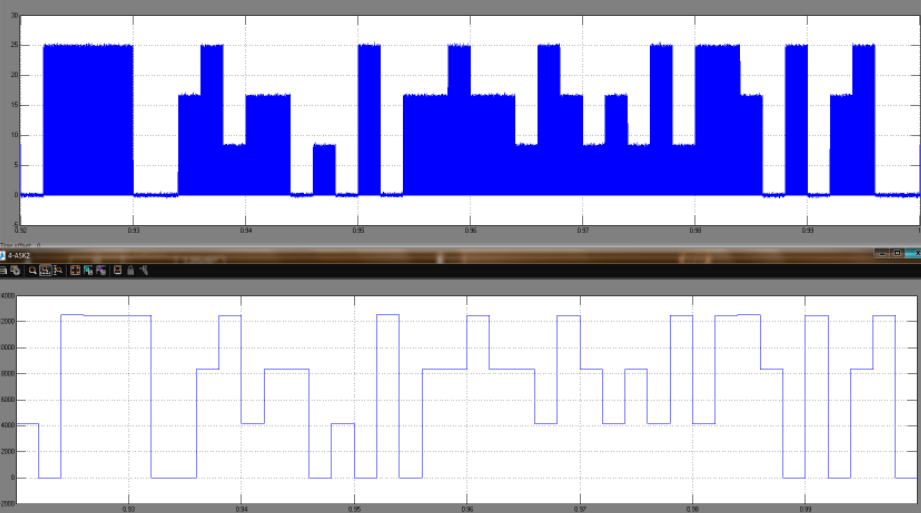
\includegraphics[scale=0.3]{rask8}
%    \caption{ASK x ASK4.}
%    \label{fig:rask8}
%\end{figure}
%
%\begin{figure}[H]
%    \centering
%    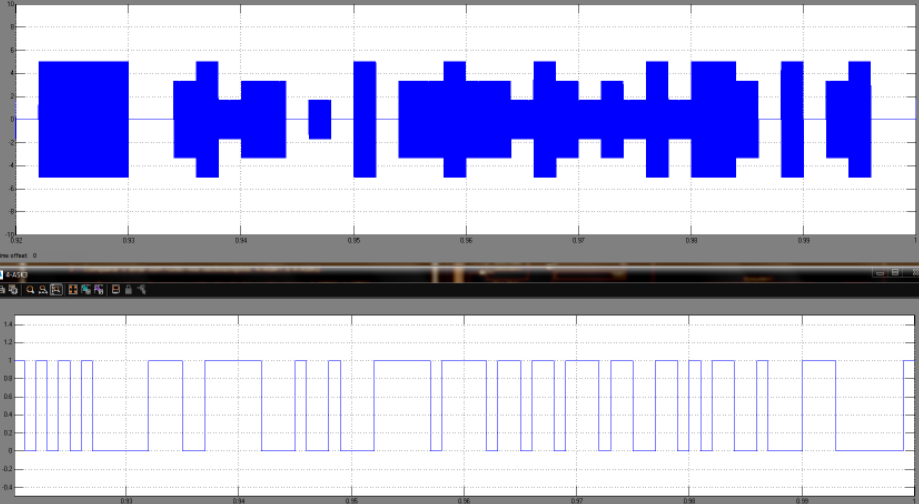
\includegraphics[scale=0.3]{rask9}
%    \caption{ASK2 x ASK1.}
%    \label{fig:rask9}
%\end{figure}
%
%Além de tudo isso já apresentado, foi obtido a PSD do esquema seguindo o modo de implementação do bloco abaixo também representado, obtendo então a banda central assim como suas frequências:
%
%\begin{figure}[H]
%    \centering
%    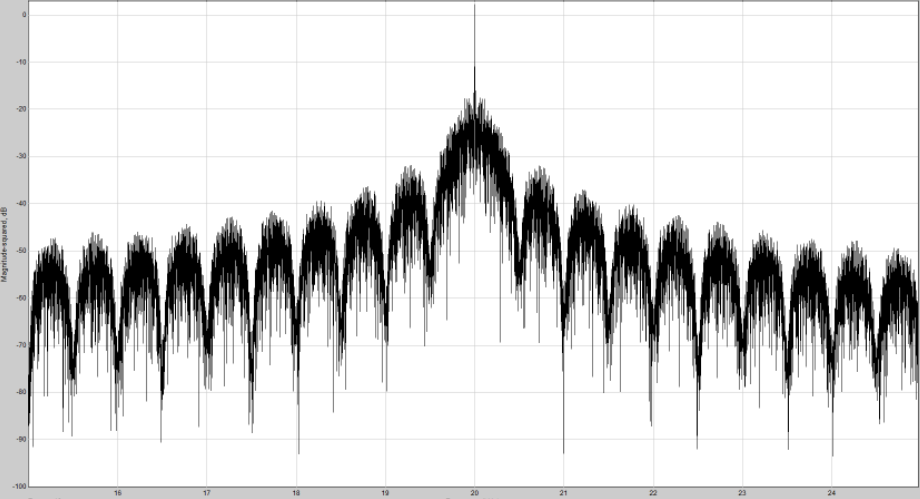
\includegraphics[scale=0.3]{rpsd-ask}
%    \caption{Densidade espectral de potência para modulação ASK.}
%    \label{fig:rpsdask}
%\end{figure}
%
%Para a obtenção do gráfico Eb/No x BER (semilog), desenvolveu-se a tabela abaixo, além de seguir a fórmula abaixo tendo uma potência do sinal de 25W:
%Para o Matlab:
%
%\begin{small}
%    \begin{table}[H]
%        \begin{center}
%            \caption{Tabela BER x Eb/No para 4-ASK com codificação \textit{Gray}.}
%            \begin{tabular}{c|c|c}
%                \hline
%                $\frac{Eb}{No}$ [dB] & BER & $P_b$ \\
%                \hline
%                14 & 0,002 & 0.0028\\
%                \hline
%                12 & 0,0108 & 0.0125\\
%                \hline
%                10 & 0,0364 & 0.0341\\
%                \hline
%                8 & 0,0654 & 0.0672\\
%                \hline
%                6 & 0,1113 & 0.1072 \\
%                \hline
%                4 & 0,1519 & 0.1488 \\
%                \hline
%                2 & 0,2019 & 0.1878 \\
%                \hline
%                0 & 0,2484 & 0.2223 \\
%                \hline
%            \end{tabular}
%            \label{tab:3}
%        \end{center}
%    \end{table}
%\end{small}
%
%\subsection{Modulação M-FSK}
%Foi colocado as ponteiras nos lugares demarcados segundo a figura \ref{fig:FSK} e obteve-se a seguinte sequência de gráficos nos pontos onde se tinha osciloscópios:
%
%\begin{figure}[H]
%    \centering
%    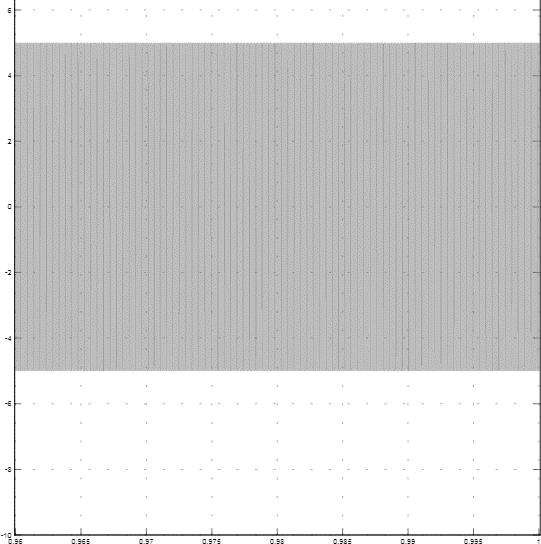
\includegraphics[scale=0.4]{rfsk1}
%    \caption{FSK.}
%    \label{fig:rpsk1}
%\end{figure}
%
%\begin{figure}[H]
%    \centering
%    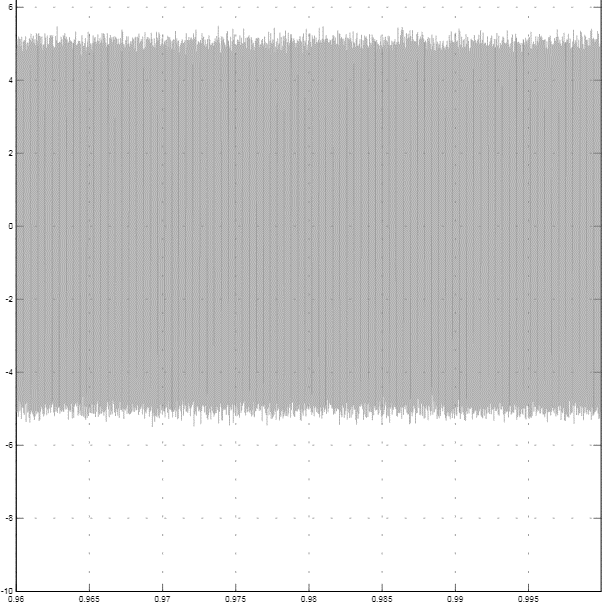
\includegraphics[scale=0.4]{rfsk2}
%    \caption{FSK1.}
%    \label{fig:rfsk2}
%\end{figure}
%
%\begin{figure}[H]
%    \centering
%    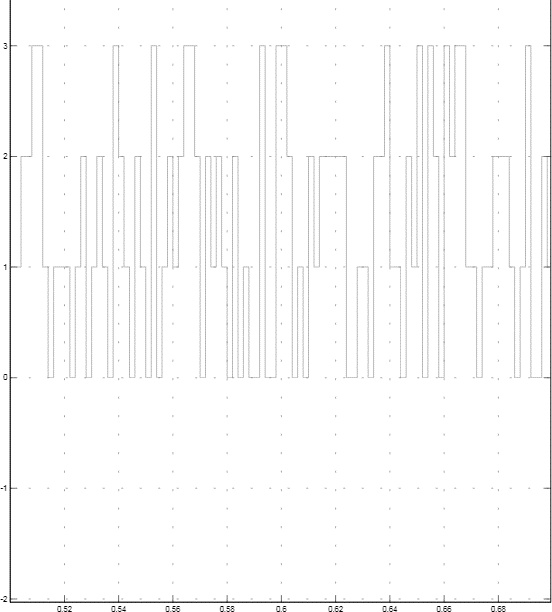
\includegraphics[scale=0.4]{rfsk3}
%    \caption{FSK2.}
%    \label{fig:rfsk3}
%\end{figure}
%
%\begin{figure}[H]
%    \centering
%    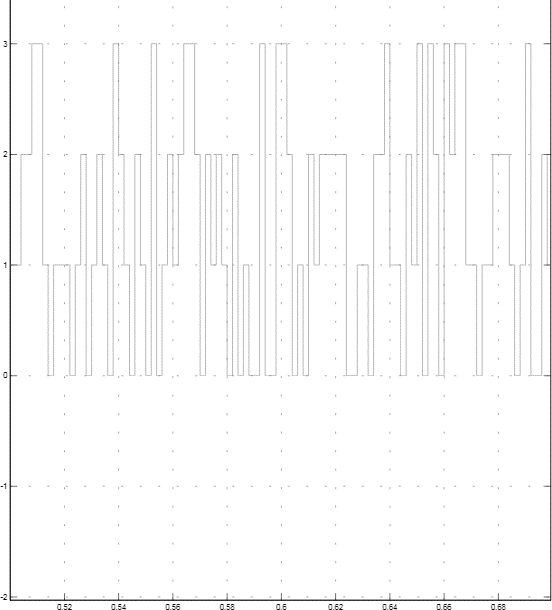
\includegraphics[scale=0.4]{rfsk4}
%    \caption{FSK3.}
%    \label{fig:rfsk4}
%\end{figure}
%
%\begin{figure}[H]
%    \centering
%    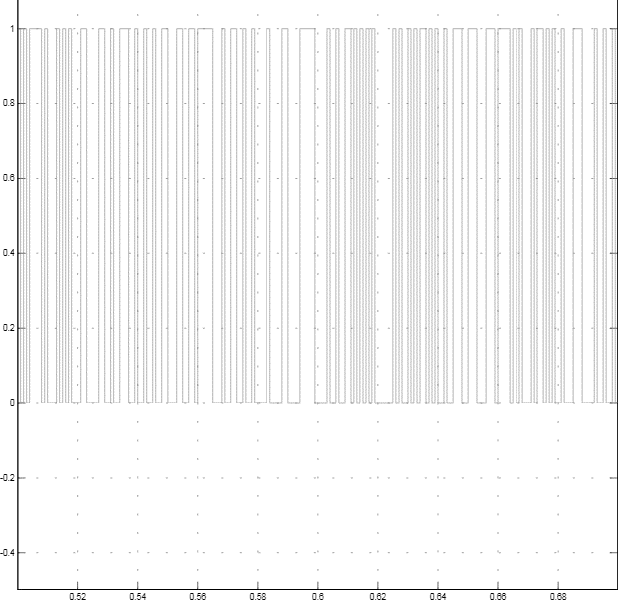
\includegraphics[scale=0.4]{rfsk5}
%    \caption{FSK4.}
%    \label{fig:rfsk5}
%\end{figure}
%
%Para ser verificado o atraso no sinal recebido em relação ao transmitido, verificou-se pela figura \ref{fig:rfsk6}, que temos um atraso de 6 bits da entrada em relação a saída:
%\begin{figure}[H]
%    \centering
%    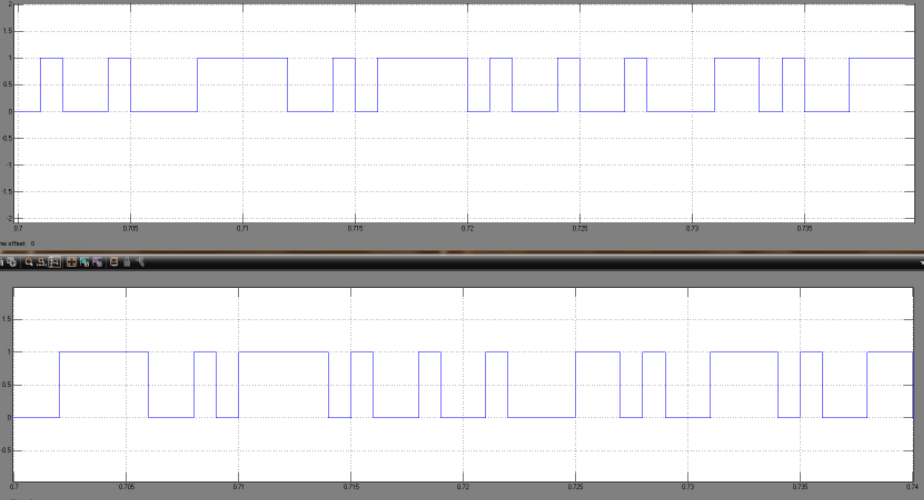
\includegraphics[scale=0.3]{rfsk6}
%    \caption{Atraso.}
%    \label{fig:rfsk6}
%\end{figure}
%
%
%Obteve-se então o seguinte gráfico relacionando os resultados práticos (BER) e os teóricos (PB), de acordo com a tabela acima apresentada:
%
%\begin{figure}[H]
%    \centering
%    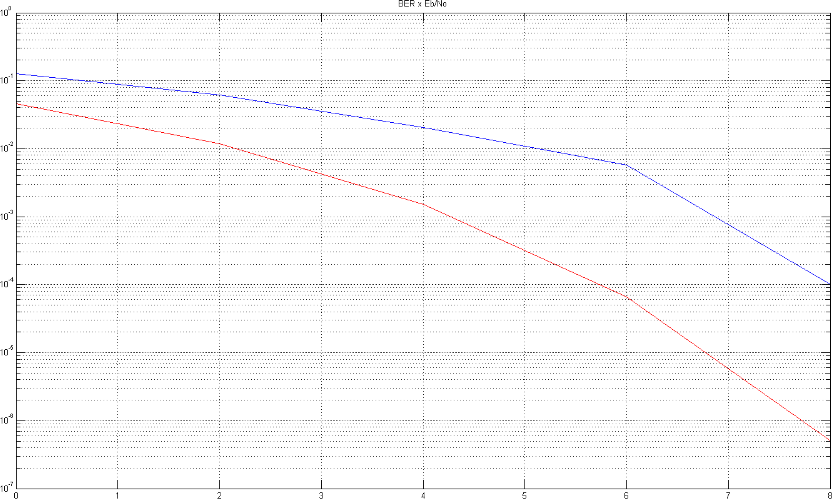
\includegraphics[scale=0.3]{rfsk7}
%    \caption{Relação BERxNo e Pb.}
%    \label{fig:rfsk7}
%\end{figure}
%
%Também encontrou-se a relação FSK com FSK4 e FSK2 com FSK1, sendo respectivamente as imagens abaixo. Esses pontos são os respectivos que provam na pratica a teoria da modulação FSK.
%
%\begin{figure}[H]
%    \centering
%    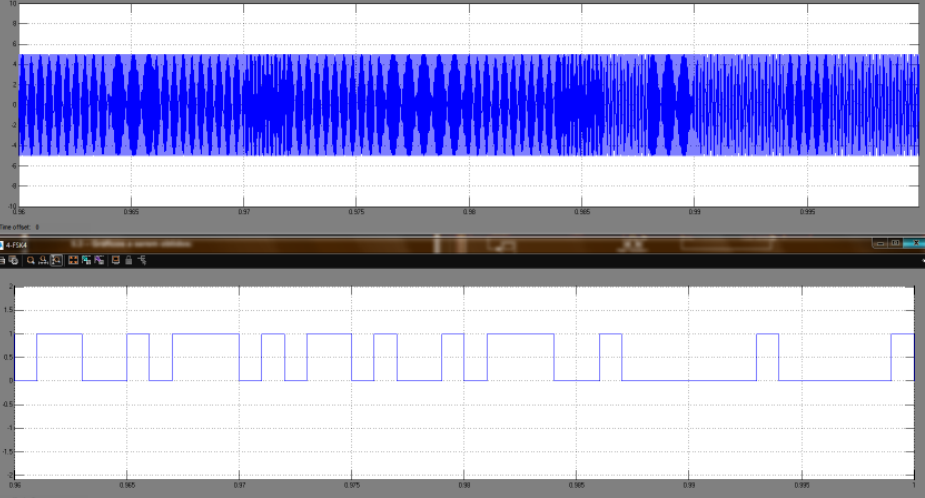
\includegraphics[scale=0.3]{rfsk8}
%    \caption{FSK x FSK4.}
%    \label{fig:rfsk8}
%\end{figure}
%
%\begin{figure}[H]
%    \centering
%    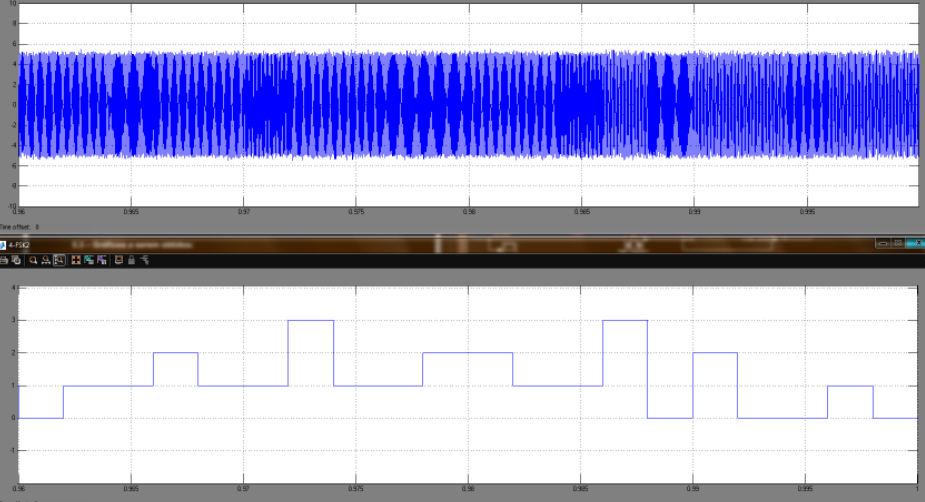
\includegraphics[scale=0.3]{rfsk9}
%    \caption{FSK2 x FSK1.}
%    \label{fig:rfsk9}
%\end{figure}
%
%Além de tudo isso já apresentado, foi obtido a PSD do esquema seguindo o modo de implementação do bloco abaixo também representado, obtendo então a banda central assim como suas frequências:
%
%\begin{figure}[H]
%    \centering
%    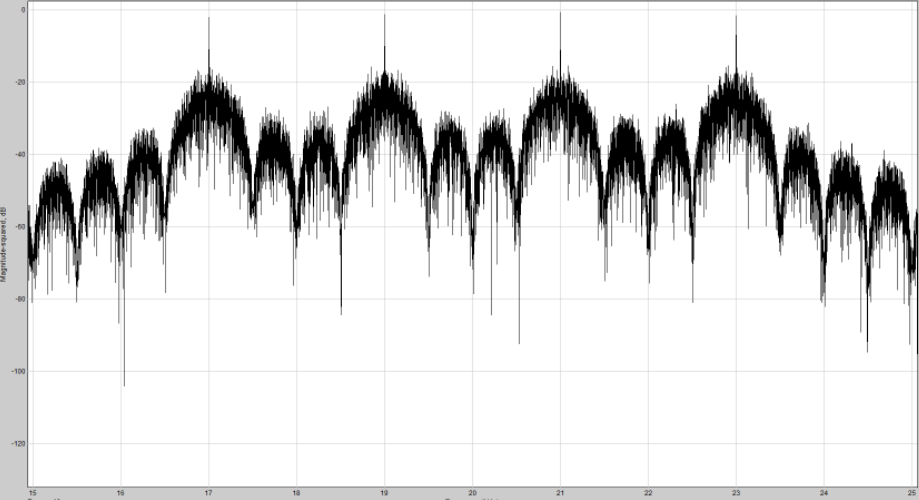
\includegraphics[scale=0.3]{rpsd-fsk}
%    \caption{Densidade espectral de potência para modulação FSK.}
%    \label{fig:rsdfsk}
%\end{figure}
%
%Para a obtenção do gráfico Eb/No x BER (semilog), desenvolveu-se a tabela abaixo, além de seguir a fórmula abaixo tendo uma potência do sinal de 25W:
%Para o Matlab:
%
%\begin{small}
%    \begin{table}[H]
%        \begin{center}
%            \caption{Tabela BER x Eb/No para 4-FSK com codificação \textit{Gray}.}
%            \begin{tabular}{c|c|c}
%                \hline
%                $\frac{Eb}{No}$ [dB] & BER & $P_b$ \\
%                \hline
%                8 & 0,0001 & 0.0004\\
%                \hline
%                6 & 0,0057 & 0.0048 \\
%                \hline
%                4 & 0,0207 & 0.0250 \\
%                \hline
%                2 & 0,0623 & 0.0750 \\
%                \hline
%                0 & 0,1262 & 0.1573 \\
%                \hline
%            \end{tabular}
%            \label{tab:3}
%        \end{center}
%    \end{table}
%\end{small}
%
%\subsection{Modulação M-PSK}
%Foi colocado as ponteiras nos lugares demarcados segundo a figura \ref{fig:PSK} e obteve-se a seguinte sequência de gráficos nos pontos onde se tinha osciloscópios:
%
%\begin{figure}[H]
%    \centering
%    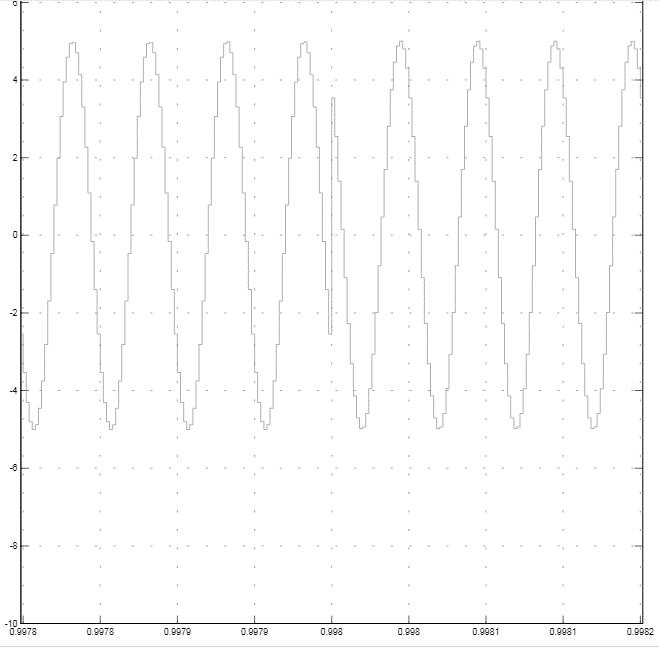
\includegraphics[scale=0.4]{rpsk1}
%    \caption{PSK.}
%    \label{fig:rpsk1}
%\end{figure}
%
%\begin{figure}[H]
%    \centering
%    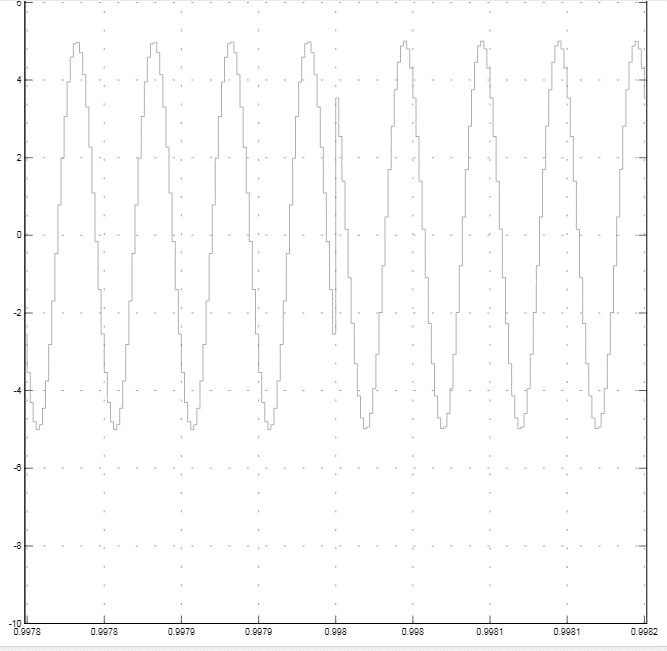
\includegraphics[scale=0.4]{rpsk2}
%    \caption{PSK1.}
%    \label{fig:rpsk2}
%\end{figure}
%
%\begin{figure}[H]
%    \centering
%    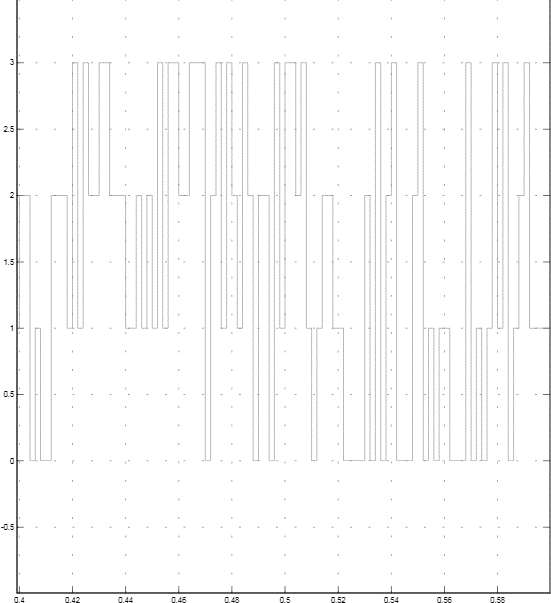
\includegraphics[scale=0.4]{rpsk3}
%    \caption{PSK2.}
%    \label{fig:rpsk3}
%\end{figure}
%
%\begin{figure}[H]
%    \centering
%    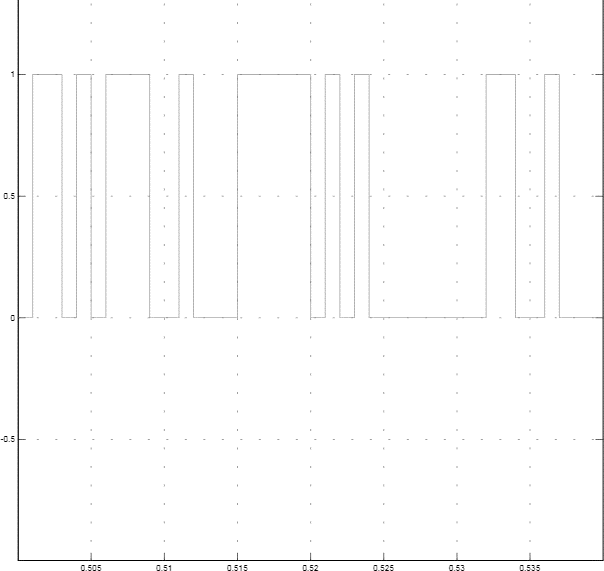
\includegraphics[scale=0.4]{rpsk4}
%    \caption{PSK3.}
%    \label{fig:rpsk4}
%\end{figure}
%
%\begin{figure}[H]
%    \centering
%    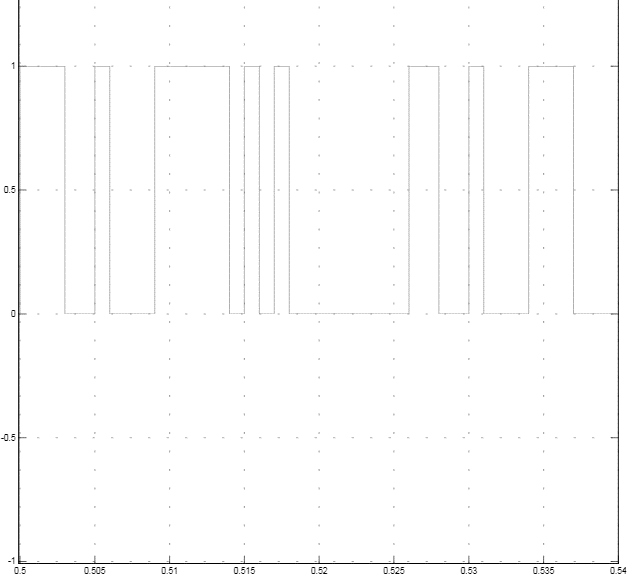
\includegraphics[scale=0.4]{rpsk5}
%    \caption{PSK4.}
%    \label{fig:rpsk5}
%\end{figure}
%
%Para ser verificado o atraso no sinal recebido em relação ao transmitido, verificou-se pela figura \ref{fig:rpsk6}, que temos um atraso de 6 bits da entrada em relação a saída:
%\begin{figure}[H]
%    \centering
%    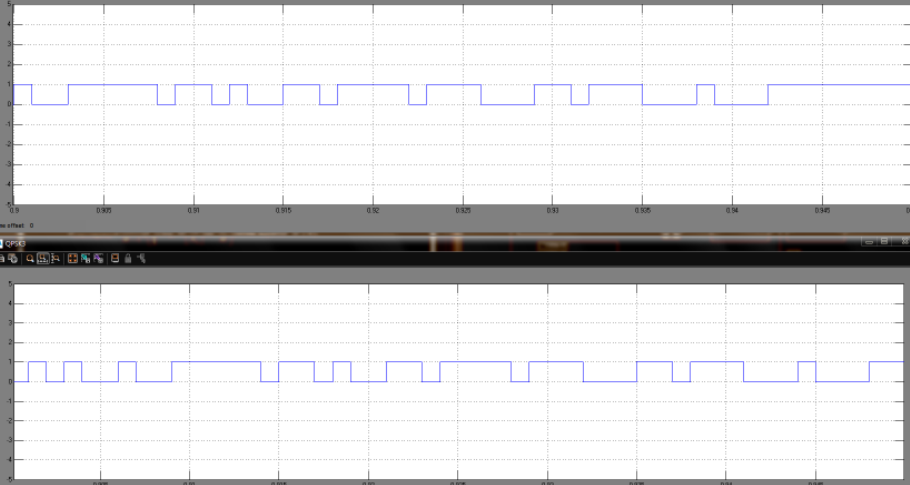
\includegraphics[scale=0.3]{rpsk6}
%    \caption{Atraso.}
%    \label{fig:rpsk6}
%\end{figure}
%
%
%Obteve-se então o seguinte gráfico relacionando os resultados práticos (BER) e os teóricos (PB), de acordo com a tabela acima apresentada:
%
%\begin{figure}[H]
%    \centering
%    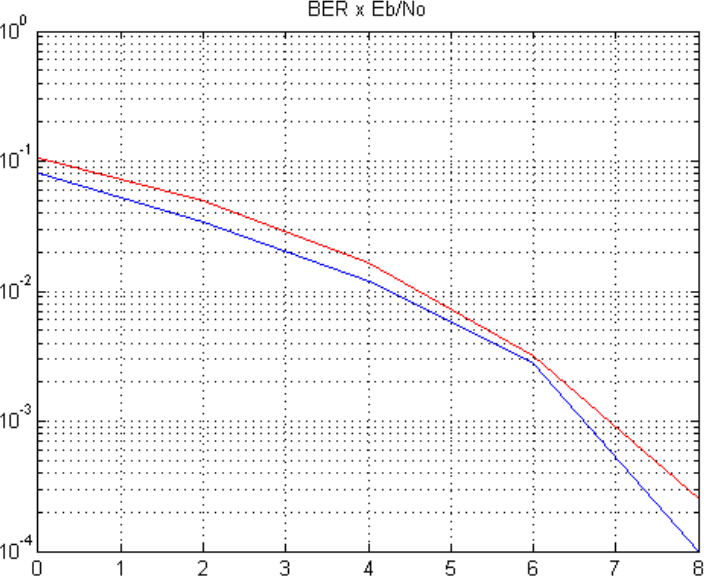
\includegraphics[scale=0.3]{rpsk7}
%    \caption{Relação BERxNo e Pb.}
%    \label{fig:rpsk7}
%\end{figure}
%
%Também encontrou-se a relação PSK com PSK4 e PSK2 com PSK1, sendo respectivamente as imagens abaixo. Esses pontos são os respectivos que provam na pratica a teoria da modulação PSK.
%
%\begin{figure}[H]
%    \centering
%    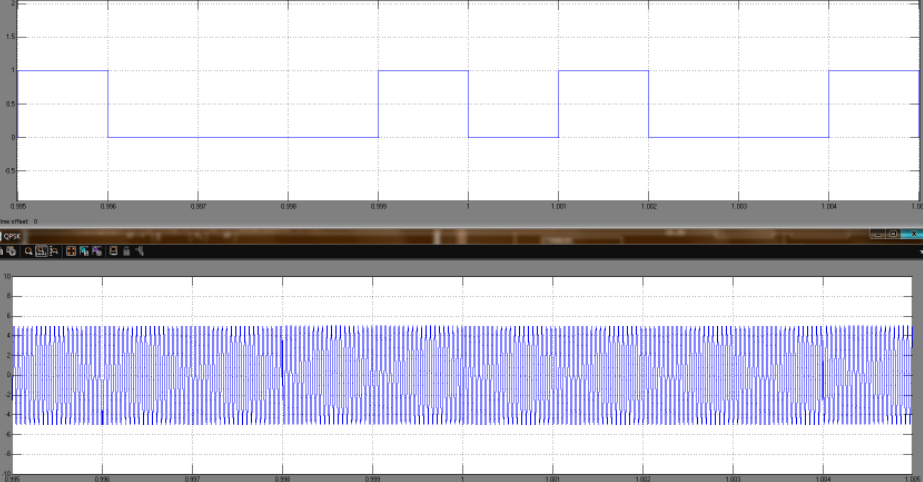
\includegraphics[scale=0.3]{rpsk8}
%    \caption{PSK x PSK4.}
%    \label{fig:rpsk8}
%\end{figure}
%
%\begin{figure}[H]
%    \centering
%    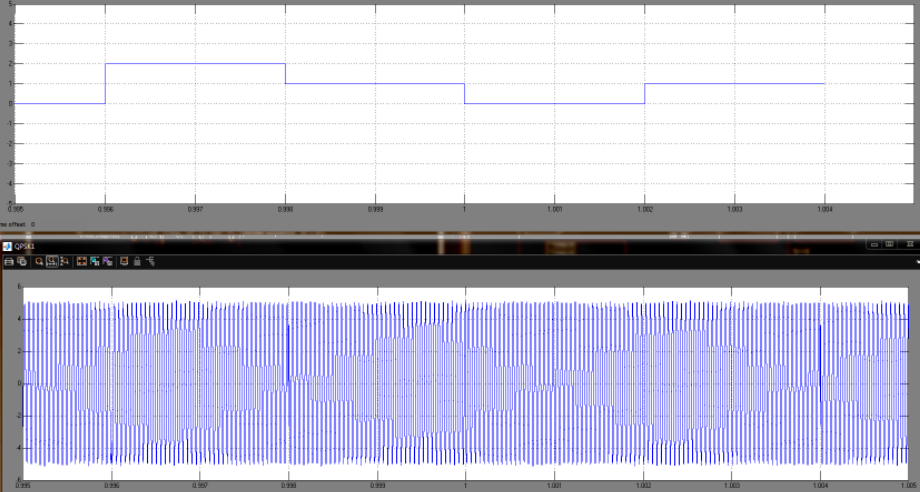
\includegraphics[scale=0.3]{rpsk9}
%    \caption{PSK2 x PSK1.}
%    \label{fig:rpsk9}
%\end{figure}
%
%Além de tudo isso já apresentado, foi obtido a PSD do esquema seguindo o modo de implementação do bloco abaixo também representado, obtendo então a banda central assim como suas frequências:
%
%\begin{figure}[H]
%    \centering
%    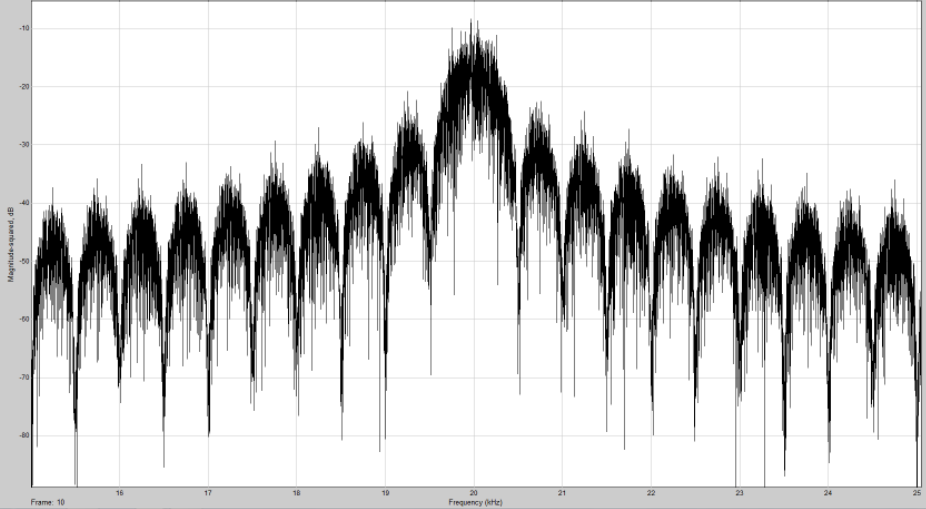
\includegraphics[scale=0.3]{rpsd-psk}
%    \caption{Densidade espectral de potência para modulação PSK.}
%    \label{fig:rpsdpsk}
%\end{figure}
%
%Para a obtenção do gráfico Eb/No x BER (semilog), desenvolveu-se a tabela abaixo, além de seguir a fórmula abaixo tendo uma potência do sinal de 25W:
%Para o Matlab:
%
%\begin{small}
%    \begin{table}[H]
%        \begin{center}
%            \caption{Tabela BER x Eb/No para 4-PSK com codificação \textit{Gray}.}
%            \begin{tabular}{c|c|c}
%                \hline
%                $\frac{Eb}{No}$ [dB] & BER & $P_b$ \\
%                \hline
%                8 & 0,0001 & 0.0003\\
%                \hline
%                6 & 0,0028 & 0.0032 \\
%                \hline
%                4 & 0,012 & 0.0167 \\
%                \hline
%                2 & 0,0338 & 0.0500 \\
%                \hline
%                0 & 0,082 & 0.1049 \\
%                \hline
%            \end{tabular}
%            \label{tab:3}
%        \end{center}
%    \end{table}
%\end{small}
%
%\subsection{Comparação entre as técnicas de modulação}
%
%Como último item do relatório, juntou-se todas as relações de BER/No de todas as modulações apresentadas para verificar qual seria a melhor, conforme a figura 
%
%\begin{figure}[H]
%    \centering
%    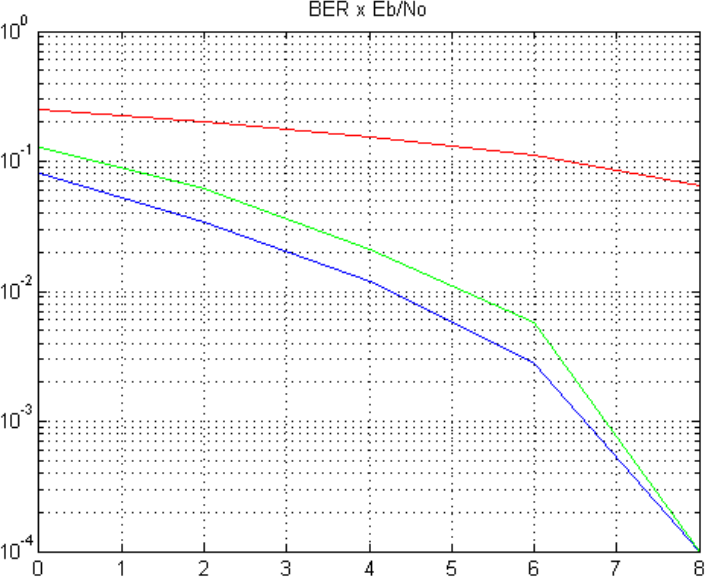
\includegraphics[scale=0.3]{bernoall}
%    \caption{Comparação entre a BER para modulação ASK, FSK e PSK.}
%    \label{fig:bernoall}
%\end{figure}